\documentclass[tikz,border=6pt]{standalone}
\usepackage[T1]{fontenc}
\usepackage{lmodern}
\usetikzlibrary{arrows.meta,positioning,shapes.geometric,fit,calc,backgrounds}
\definecolor{ink}{HTML}{292642}
\definecolor{violet}{HTML}{7054DC}
\definecolor{violetlight}{HTML}{F1EDFF}
\definecolor{teal}{HTML}{147D77}
\definecolor{teallight}{HTML}{E8F5F3}
\definecolor{amber}{HTML}{9A641F}
\definecolor{amberlight}{HTML}{FFF3DE}
\definecolor{linegray}{HTML}{A7A9BA}
\tikzset{box/.style={draw=violet!55,fill=violetlight,rounded corners=3pt,minimum width=2.25cm,minimum height=0.8cm,align=center,font=\sffamily\scriptsize,text=ink,inner sep=5pt},actual/.style={box,draw=teal!70,fill=teallight},proposed/.style={box,dashed,draw=amber!75,fill=amberlight},small/.style={font=\sffamily\tiny,text=ink,align=center},lab/.style={font=\sffamily\scriptsize\bfseries,text=ink},flow/.style={-{Stealth[length=2mm]},line width=.8pt,draw=violet},dflow/.style={flow,dashed,draw=amber},boundary/.style={draw=linegray,dashed,rounded corners=4pt,inner sep=8pt}}
\begin{document}

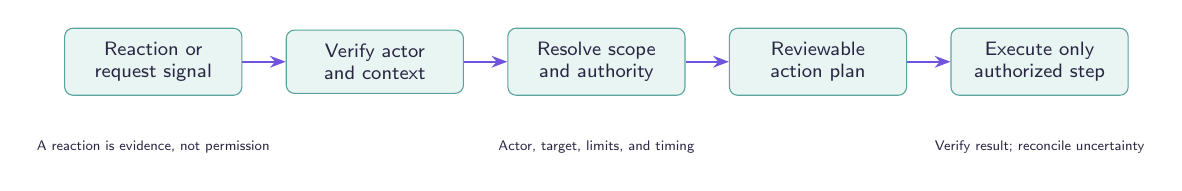
\begin{tikzpicture}[node distance=.65cm and .55cm]
\node[actual] (signal) {Reaction or\\request signal};
\node[actual,right=of signal] (actor) {Verify actor\\and context};
\node[actual,right=of actor] (scope) {Resolve scope\\and authority};
\node[actual,right=of scope] (plan) {Reviewable\\action plan};
\node[actual,right=of plan] (exec) {Execute only\\authorized step};
\draw[flow] (signal)--(actor);\draw[flow] (actor)--(scope);\draw[flow] (scope)--(plan);\draw[flow] (plan)--(exec);
\node[small,below=.45cm of signal] {A reaction is evidence, not permission};
\node[small,below=.45cm of scope] {Actor, target, limits, and timing};
\node[small,below=.45cm of exec] {Verify result; reconcile uncertainty};
\end{tikzpicture}
\end{document}
